%!TEX root = ../report.tex

\begin{document}
    \chapter{State of the Art}
	\label{chap:stateofart}
	
	Introduction to modern deep learning and their impact on the various vision tasks are described in the \nameref{sec:deeplearn} section. Information fusion in the temporal domain to fuse information is explained in \nameref{sec:tempfuse}. State-of-the-art segmentation of the input images, in particular, the semantic segmentation task, is illustrated in the \nameref{sec:semseg} section. State-of-the-art segmentation in the classical era and modern deep learning plays a crucial role in temporally fused semantic segmentation. However, there is very little work in fusing the camera pose into the segmentation task in a temporal fashion. More details are discussed in the \nameref{sec:semseg}. Finally, chapter \ref{chap:stateofart} is ended with a discussion on the limitations of the previous work concerning temporal fusion. 
	
    \section{Deep Learning}
    \label{sec:deeplearn}
    
	Deep learning is a subfield of machine learning that aims to learn the features present in the data by utilizing hierarchical architectures. The deep area learning falls in artificial intelligence is depicted in the picture \ref{fig:DLAI}
    
    \begin{figure}[h]
    	\centering
    	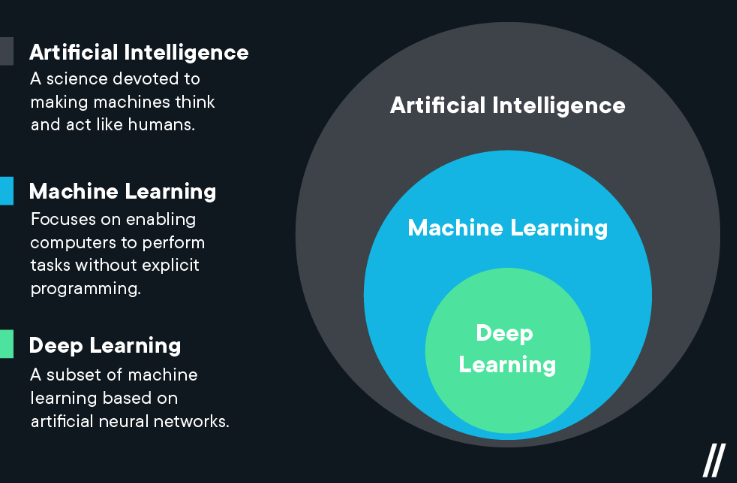
\includegraphics[width=10cm]{images/mldl.png}
    	\caption{Deep learning in the artificial intelligence domain. Courtesy of \cite{35_mldl}}
    	\label{fig:DLAI}
    \end{figure}  
    
    Classical machine learning system uses the raw input, and domain experts carefully represent the data as a feature vector from which the data is fed to the models to learn the patterns and classify them into appropriate classes \cite{36_lecun2015deep}. 
    Deep learning is a representation learning that takes raw data and finds the patterns in the data with different levels of representation in the multiple layers \cite{36_lecun2015deep}. Deep learning can learn any complex representation of the data. For example, an image is represented as pixels and is fed to the neural network; at each layer of the network, a different feature is learned. Higher-level features, such as edges at a specific orientation and location, are determined in the first layer. In the second layer, motifs are learned, and so on. The vital aspect of deep learning is that the features are not designed by the field expert but instead learned from the data with a specific set of learning procedures \cite{36_lecun2015deep}.
    
	Many current state-of-the-art learning models use the deep learning approach to learn a complex function from data. Currently, deep learning methods can be found in image recognition \cite{37_farabet2012learning}, speech technologies \cite{38_hinton2012deep}, the discovery of drug molecule \cite{39_patel2020machine}, understanding the particle accelerator data \cite{40_ciodaro2012online}, DNA sequencing \cite{41_zhang2021deep}, and natural language processing \cite{42_hirschberg2015advances}. 
    
    Computer vision is the field of computer science that deals with replicating the functionalities of the human visual system. Traditionally computer vision solved the vision problem by finding hand-crafted features. However, the performance of the classical approach is outperformed by the advancement of deep learning-based methods. Hand-crafted feature descriptors such as Speeded Up Robust Features (SURF) and Hough Transforms are used as feature vectors for the classical machine learning methods for learning \cite{46_o2019deep}. Deep learning methods automatically learn the patterns from the data. Computer vision solves a wide variety of problems in the perception domain. Latest approaches helps to solve the detection \cite{44_mohanty2016using}, \cite{45_han2021ecological}, classification \cite{43_srivastava2021comparative}, image synthesis and segmentation tasks \cite{47_minaee2021image}.
    
	Temporal data are time-varying information and can be commonly observed in financial portfolio management, accounting, medical records, inventory management, and data from the airline, hotel; train industries contain time components with it \cite{48_jensen1999temporal}. Video data are constructed by combining time variant frames and are a typical example of temporal data. Temporal fusion deals with combining past information into the current step computation with the aim of improved performance. 
    
	In general, approach segmentation is done frame by frame or by skipping between frames and computing the segmentation on the nth frame. Temporal fusion can be applied in these settings to improve segmentation by combining the past rich information in the current step. 
     
    \section{Temporal Fusion}
    \label{sec:tempfuse}
    
	Temporal fusion can be defined as the process of fusing the temporal data onto the current step to improve the model's performance. Temporal data can be observed in many fields, such as social media, healthcare, accounting, agriculture, transportation, physics, crime data, traffic dynamics, and climate science \cite{49_atluri2018spatio}. Temporal data can be encountered with different data types: video, audio, tabular data, and sensor data. Forecasting is a typical application of temporal fusion. Multi-horizon forecasting is an important problem in the domain of time series. Multi-horizon forecasts allow the user to optimize the process across the entire path. A novel Temporal fusion Transformer (TFT) \cite{50_lim2021temporal} is an attention-based DNN architecture for forecasting by fusing the important past features into the current step. Temporal fusion plays a significant role in improved video action recognition. Temporal fusion helps in two ways; firstly, by understanding the temporal data, the accuracy of the recognition for the dynamic action is improved; secondly, removing the redundant temporal data saves the computation overhead. A temporal fusion network known as the AdaFuse fuses the current and past features with a goal of improved accuracy and efficiency \cite{51_meng2021adafuse}. A temporal nonparametric fusion aims to fuse the temporal pose data to the computation of the depth map, thereby improving accuracy and efficiency \cite{52_hou2019multi}. The architecture of the multi-view stereo can be depicted in Fig \ref{fig:mvs}. An online multi-view depth prediction approach where the depth estimated in the previous step is fused onto the current step in a sensible manner. The network is named DeepVideoMVS, and it is based on the encoder-decoder architecture. A ConvLSTM is placed at the latent space to fuse the information from the previous step. The proposed approach outperformed all the existing state-of-the-art multi-view stereo methods evaluated on the standard metrics \cite{53_duzceker2021deepvideomvs}. 
	A Multiple Fusion Adaptation (MFA) method improves the segmentation accuracy on an unlabeled dataset. Three fusion approach was proposed under MFA, cross-model fusion, temporal fusion, and novel online-offline pseudo labels. The MFA produced improved semantic segmentation results of 58.2\% and 62.5\% on GTA5-to-Cityscapes and SYNTHIA-to-Cityscapes, respectively \cite{54_zhang2021multiple}.  
    
    \begin{figure}
    	\centering
    	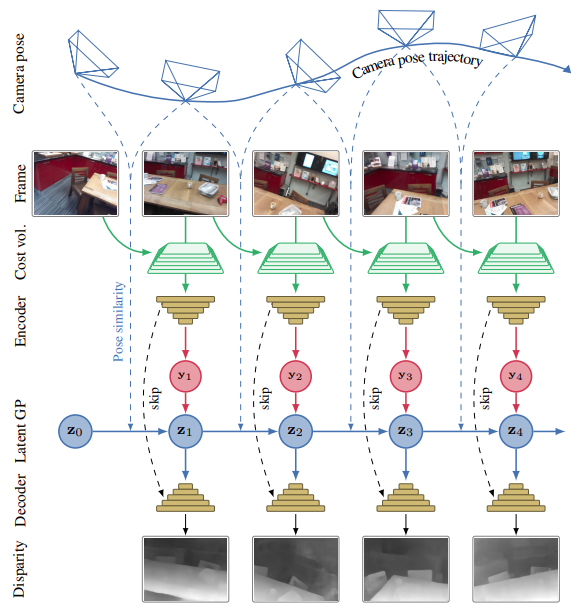
\includegraphics[width=6cm]{images/MVS.png}
    	\caption{Mulit view stereo architecture for depth estimation. Courtesy of \cite{52_hou2019multi}}
    	\label{fig:mvs}
    \end{figure} 	

    \section{Semantic Segmentation}
    \label{sec:semseg}
    
    Humans can perceive the surrounding environment and make sense of it with high accuracy. Due to the advancement of computer vision, these capabilities are transferred to machines, performing even better than humans. Today, we have computer vision models that can detect objects, find shapes, track object movement and perform an action based on the data. Computer vision is most commonly used in autonomous driving cars, aerial mapping, surveillance applications, virtual and augmented reality, etc. One common problem in computer vision is labeling each pixel of the image to a particular category. Also known as segmentation. Mathematically image segmentation can be defined as

	If $I$ is a set of all image pixels of an image, then segmentation generates unique regions ${S_1, S_2, S_3, S_4,....S_n}$ such that combining all these regions will return $I$. 
	
	Image segmentation can be classified into three categories Semantic segmentation, Instance segmentation, and Panoptic segmentation. 
	Semantic segmentation finds the objects' shape, size, and form in addition to their location. Instance segmentation finds one more parameter of a number of unique objects in the image. Panoptic segmentation is the combination of semantic and instance segmentation. The difference between all the types of semantic segmentation can be observed in Fig \ref{fig:SS}.
    
    \begin{figure}[h]
    	\centering
    	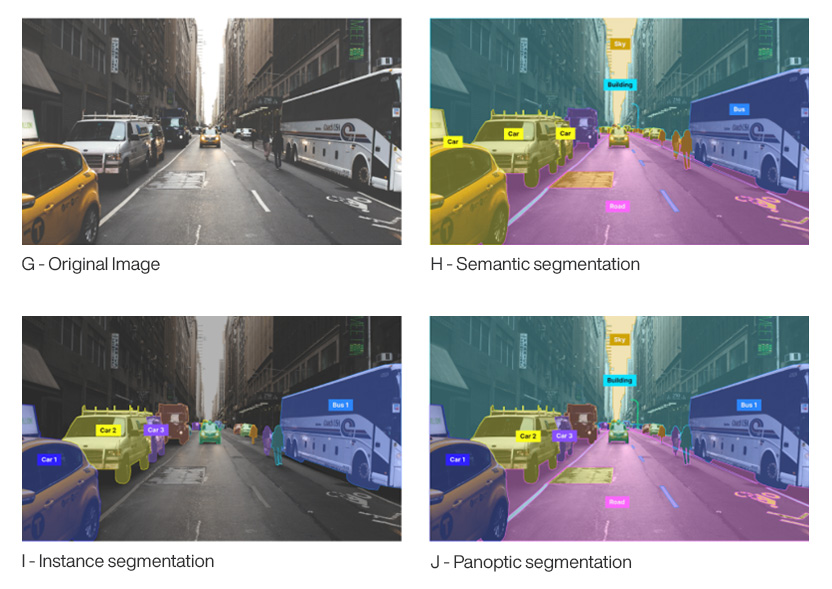
\includegraphics[width=12cm]{images/ss.jpg}
    	\caption{Semantic and Instance segmentation example. Courtesy of \cite{55_WinNT}}
    	\label{fig:SS}
    \end{figure}
    
    \subsection{Classical Semantic Segmentation}
    
	 Most commonly used traditional segmentation techniques are threshold-based technique \cite{56_otsu1979threshold}, histogram-based bundling, region-growing \cite{57_otsu1979threshold}, k-means clustering, watersheds, active contours, graph cuts, conditional and Markov random fields \cite{58_boykov2001fast}, sparsity-based methods \cite{59_starck2005image}. However, deep learning (DL) in recent years yielded a new generation of image segmentation models with state-of-the-art performance. 
    
    \subsection{Deep Learning based  Semantic Segmentation}
    
    Deep learning based segmentation network can be classified into following categories \cite{60_minaee2021image}
    
    \begin{itemize}
		\item Fully convolutional networks
		\item Convolutional models with graphical models
		\item Encoder-decoder-based models
		\item Multi-scale and pyramid network-based models
		\item R-CNN-based models (for instance segmentation)
		\item Dilated convolutional models and DeepLab family
		\item Recurrent neural network-based models
		\item Attention-based models
		\item Generative models and adversarial training
		\item Convolutional models with active contour models
	\end{itemize}
    
    Deep learning-based computer vision models most commonly use the convolutional neural network \cite{61_chen2017rethinking}, recurrent neural network (RNNs), and Long short term memory (LSTM), encoder-decoder \cite{62_badrinarayanan2017segnet}. Generative adversarial networks (GANs) based networks \cite{60_minaee2021image}. The master thesis work is concentrated on the encoder-decoder-based deep learning models. The encoder-Decoder-based network is a two-stage network that learns to map from the input point to the output point. In the encoder stage, the input data is compressed into a latent space representation $ z = f(x)$ and the decoder decompresses the latent space representation to the output $ a = g(z)$ \cite{63_goodfellow2014generative}. Latent representation of the input data in compressed form. It can be commonly observed in image-to-image translation problems and in sequence-to-sequence models in NLP. A reconstruction loss $ L(y, \hat{y})$ is defined at the output that measures the differences between the ground truth output $y$ and corresponding reconstruction $\hat{y}$. Autoencoders are the particular version of the encoder-decoder models with similar input and output.
    
    \begin{figure}[h]
    	\centering
    	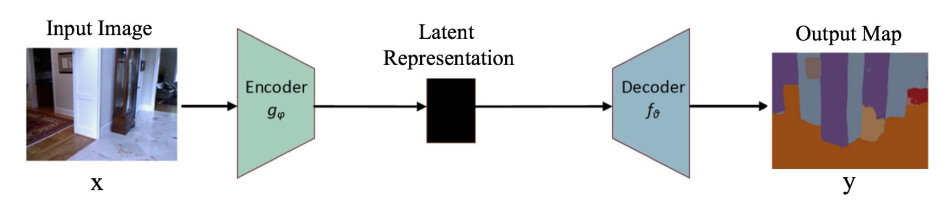
\includegraphics[width=14cm]{images/en_de.png}
    	\caption{Simple encoder-decoder architecture. Courtesy of \cite{60_minaee2021image}}
    	\label{fig:en_de}
    \end{figure} 		
    
	Most of the segmentation networks are encoder-decoder-based architecture. A novel semantic segmentation network was proposed by Noh et al. \cite{64_noh2015learning}. The network is based on deconvolution. The encoder network is based on the VGG 16-layer network, and the decoder network takes the latent space encoding and outputs the pixel-wise class probabilities. The segmentation mask and pixel-wise class labels are predicted by the deconvolutional and unpooling layers. The network generated an accuracy of 72.5 \% on the PASCAL VOC 2012 dataset. 
    
    \begin{figure}[h]
    	\centering
    	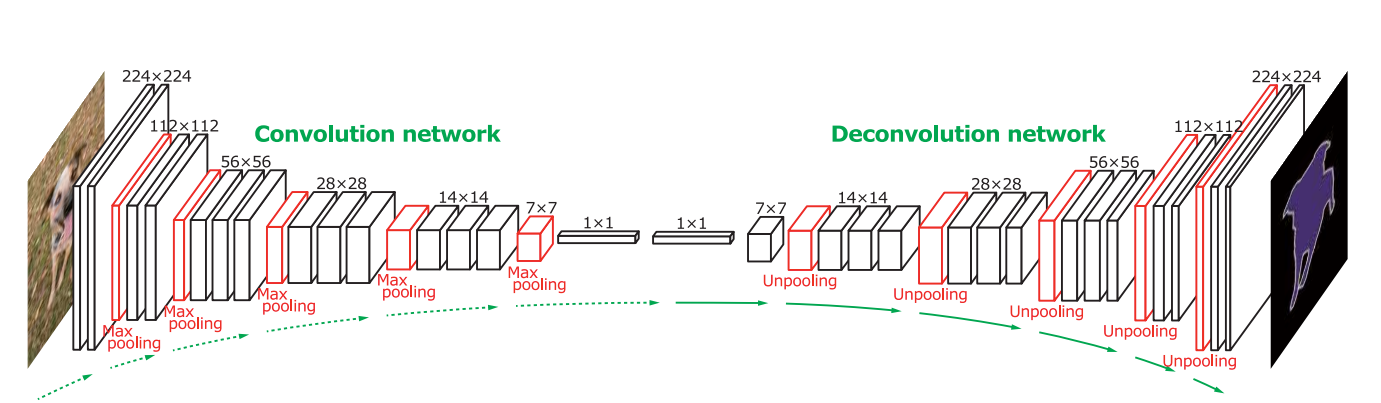
\includegraphics[width=14cm]{images/general_seg.png}
    	\caption{Simple encoder-decoder architecture. Courtesy of \cite{64_noh2015learning}}
    	\label{fig:general_seg}
    \end{figure} 
    
    Badrinarayanan et al proposed a convolutional encoder-decoder architecture for image segmentation called as SegNet \cite{62_badrinarayanan2017segnet}. The architecture of the SegNet described in the Figure \ref{fig:segnet}  
    
    \begin{figure}[h]
    	\centering
    	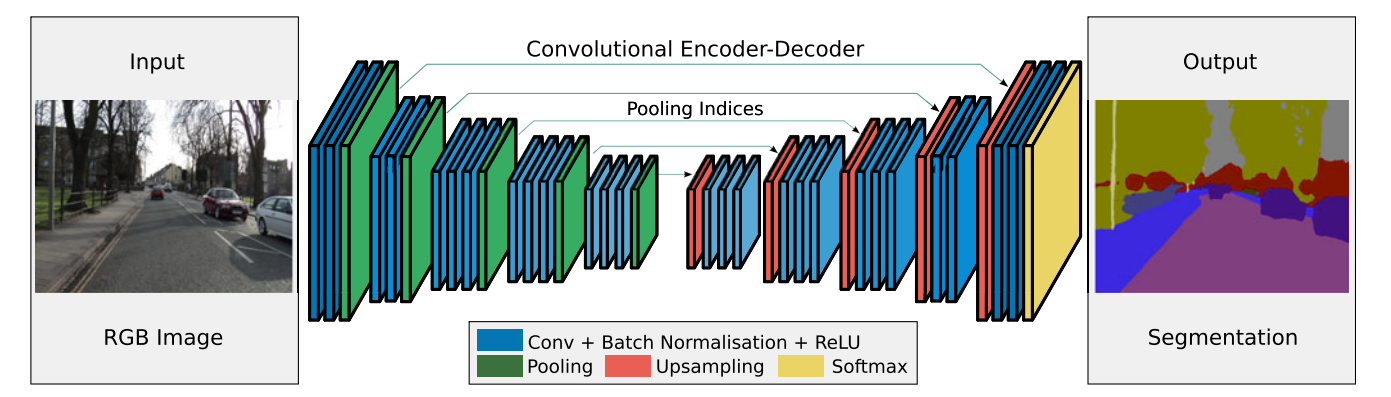
\includegraphics[width=14cm]{images/segnet.png}
    	\caption{SegNet architecture. Courtesy of \cite{62_badrinarayanan2017segnet}}
    	\label{fig:segnet}
    \end{figure} 
    
    The encoder part of the SegNet consists of 13 convolutional layers in the VGG16 network, followed by the pixel-wise classification layer. Decoder uniquely upsamples the low-resolution feature maps. Non-linear upsampling is performed by using the pooling indices computed in the max-pooling step of the encoder. This process of reusing the encoder output helps to eliminate the need for learning to up-sample. Dense feature maps are generated by convolving with the trainable filters. To account for the uncertainty involved with the encoder-decoder network, scene segmentation is proposed \cite{65_kendall2015bayesian}. HRNet \cite{66_sun2019high} is the recently developed high-resolution network that connects the high to low-resolution convolutions streams in parallel	and exchanges information between different resolutions. HRNet maintains high-resolution representation through the encoding process. Many recent architectures use HRNet as the backbone. Other encoder decoder segmentation models are Stacked Deconvolutional Network \cite{67_fu2019stacked}, Linknet \cite{68_hu2018learning}, W-net \cite{69_xia2017w}.

	Many segmentation models are developed for medical applications, and among those, U-Net \cite{70_ronneberger2015u}, and V-Net \cite{71_milletari2016v} are the famous architecture. These architectures are now used outside of the medical domain.
    
    \begin{figure}[h]
    	\centering
    	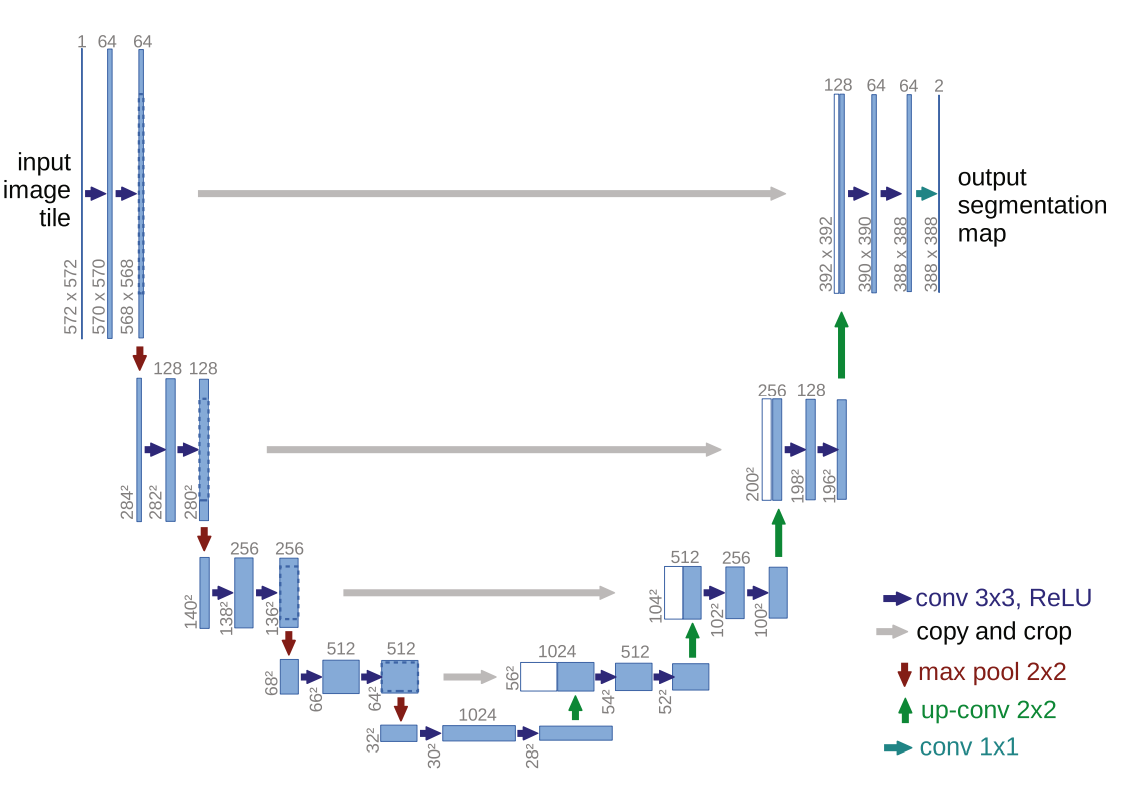
\includegraphics[width=14cm]{images/unet.png}
    	\caption{Unet architecture. Courtesy of \cite{70_ronneberger2015u}}
    	\label{fig:unet}
    \end{figure} 
	
	 Ronneberger et al. \cite{70_ronneberger2015u} proposed a segmentation model to perform semantic segmentation on medical microscopy images. The architecture of the U-Net is described in Fig \ref{fig:unet}. The contracting part captures the context, and the expanding decoder path identifies the localization of the target area. The network heavily dependent on the annotated images efficiently. The encoder part has a 3x3 convolution features extractor, similar to the FCN-like architecture. The decoder part increases the dimensions and reduces the number of feature maps. The feature map from the encoder is mapped to the upscaled decoder to retain the pattern information. A 1x1 convolution at the output process the feature maps to generate segmentation output by categorizing each pixel of the input image to a particular class. Original U-Net was trained on the electronic microscopic images and outperformed by a large margin on the ISBI challenge. The network is fast and produces a result on 512x512 images in less than a second on the modern GPU \cite{70_ronneberger2015u}, \cite{60_minaee2021image}. In sequence data, the information from the previous frames can be utilized to segment the current frame with the aim of improved performance compared to the segmentation without the temporal fusion. 
	 
    \section{Temporal Fusion in Semantic Segmentation}
    
	Semantic segmentation of sequence data aims to assign pixel-wise semantic labels to the video frames. It is an essential task in visual understanding \cite{72_jin2017video}. A strong representation of the feature map is essential for the segmentation task. One common video segmentation approach is performing the image segmentation to each frame independently. However, this approach needs to capture the temporal information of the dynamic scenes. A standard solution to the problem is to apply semantic segmentation to every frame and add a layer on top to capture the temporal data to extract the better features \cite{73_gadde2017semantic}, \cite{74_jin2017video}, \cite{75_nilsson2018semantic}. However, such an approach does not help improve the performance as the feature needs to be computed at every frame. So a good approach is to apply the segmentation at keyframes and reuse the already computed features for the other frames \cite{76_jain2019accel}, \cite{77_mahasseni2017budget}. A new highly efficient and low accuracy neural network-based model is developed for semantic video segmentation called Temporally Distributed Network (TDNet) \cite{78_hu2020temporally}. In the TDNet feature, extraction is distributed evenly across the sequential frames to eliminate the re-computation. Then these features are combined using the Attention Propagation Module (APM) to get the solid features for accurate segmentation \cite{78_hu2020temporally}. The pictorial representation of the same is described in Fig \ref{fig:TDNet}. 
    
    \begin{figure}[h]
    	\centering
    	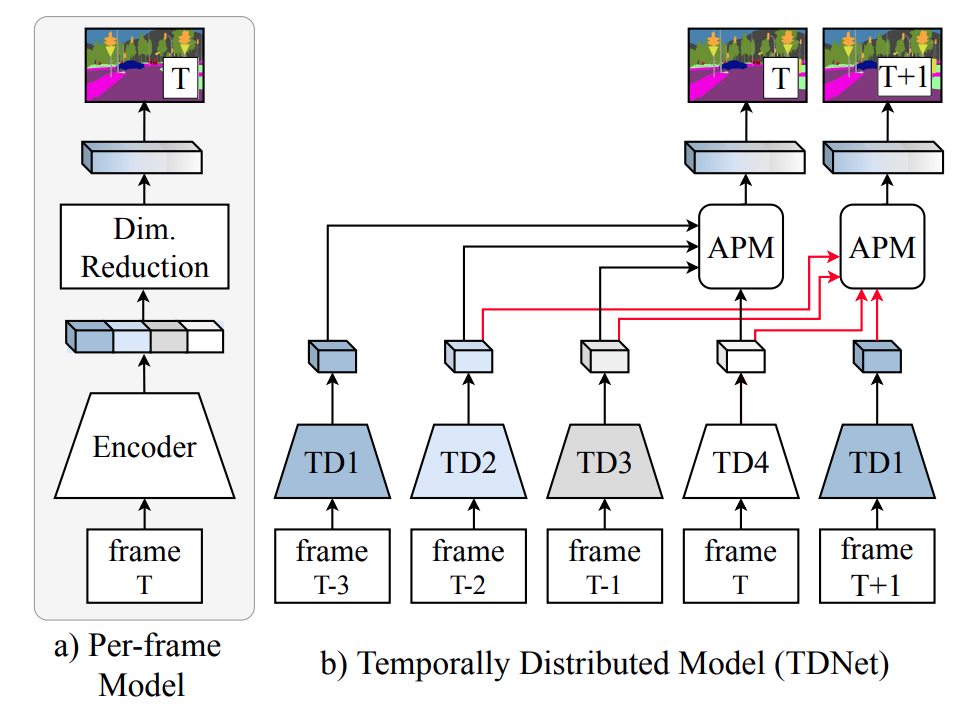
\includegraphics[width=12cm]{images/TDNet.png}
    	\caption{TDNet. Courtesy of \cite{78_hu2020temporally}}
    	\label{fig:TDNet}
    \end{figure}  
    
    \section{Limitations of Previous Work}
    
    The perception system of the modern ADAS uses segmentation to understand the surrounding environment by capturing the environment with the help of modern cameras. The high FPS data collected by the camera are in a continuous sequence where every frame is related to its previous frames. In general, setting segmentation is performed on these frames to understand the object and its boundaries, the number of objects, types of objects present in the frame. A work by Hou et al. \cite{52_hou2019multi} integrates the camera pose data into the computation of the depth maps; however, a similar strategy is not studied for a segmentation task. Also, the study of temporal data fusion in the latent space using LSTM is not studied in any previous work. This thesis aims to study the impact of temporal pose data on the computation of the semantic segmentation and to take the previous frame data onto the current frame semantic segmentation task using the LSTM network is studied. 
    
\end{document}
